


\tikzset{every picture/.style={line width=0.75pt}} %set default line width to 0.75pt        

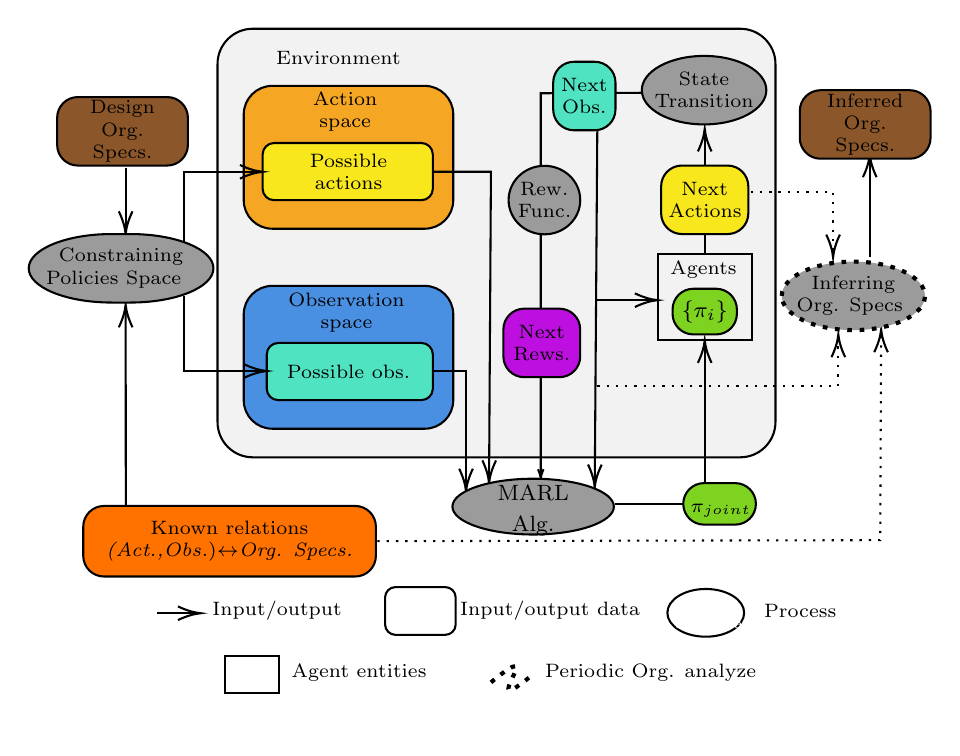
\begin{tikzpicture}[x=0.75pt,y=0.75pt,yscale=-1,xscale=1]
%uncomment if require: \path (0,1124); %set diagram left start at 0, and has height of 1124

%Shape: Rectangle [id:dp9937795244635512] 
\draw  [fill={rgb, 255:red, 242; green, 242; blue, 242 }  ,fill opacity=1 ] (108.97,721) .. controls (108.97,711.61) and (116.58,704) .. (125.97,704) -- (360.78,704) .. controls (370.17,704) and (377.78,711.61) .. (377.78,721) -- (377.78,893.49) .. controls (377.78,902.88) and (370.17,910.49) .. (360.78,910.49) -- (125.97,910.49) .. controls (116.58,910.49) and (108.97,902.88) .. (108.97,893.49) -- cycle ;
%Straight Lines [id:da6518751125509914] 
\draw    (335.62,932.92) -- (300.7,932.92) ;
%Straight Lines [id:da34207082497735786] 
\draw    (313,734.86) -- (264.7,735.09) -- (264.7,918.61) ;
\draw [shift={(264.7,920.61)}, rotate = 270] [color={rgb, 255:red, 0; green, 0; blue, 0 }  ][line width=0.75]    (4.37,-1.32) .. controls (2.78,-0.56) and (1.32,-0.12) .. (0,0) .. controls (1.32,0.12) and (2.78,0.56) .. (4.37,1.32)   ;
%Straight Lines [id:da9417034389402881] 
\draw    (343.7,754.18) -- (343.7,812.75) ;
\draw [shift={(343.7,752.18)}, rotate = 90] [color={rgb, 255:red, 0; green, 0; blue, 0 }  ][line width=0.75]    (10.93,-3.29) .. controls (6.95,-1.4) and (3.31,-0.3) .. (0,0) .. controls (3.31,0.3) and (6.95,1.4) .. (10.93,3.29)   ;
%Straight Lines [id:da4463435210078386] 
\draw    (343.7,922.88) -- (343.7,856.05) ;
\draw [shift={(343.7,854.05)}, rotate = 90] [color={rgb, 255:red, 0; green, 0; blue, 0 }  ][line width=0.75]    (10.93,-3.29) .. controls (6.95,-1.4) and (3.31,-0.3) .. (0,0) .. controls (3.31,0.3) and (6.95,1.4) .. (10.93,3.29)   ;
%Straight Lines [id:da8247669117759437] 
\draw    (291.96,834.78) -- (300.52,834.78) -- (318.99,834.78) ;
\draw [shift={(320.99,834.78)}, rotate = 180] [color={rgb, 255:red, 0; green, 0; blue, 0 }  ][line width=0.75]    (10.93,-3.29) .. controls (6.95,-1.4) and (3.31,-0.3) .. (0,0) .. controls (3.31,0.3) and (6.95,1.4) .. (10.93,3.29)   ;
%Rounded Rect [id:dp13052707912371297] 
\draw  [fill={rgb, 255:red, 245; green, 166; blue, 35 }  ,fill opacity=1 ] (121.59,745.3) .. controls (121.59,737.7) and (127.75,731.53) .. (135.35,731.53) -- (208.78,731.53) .. controls (216.39,731.53) and (222.55,737.7) .. (222.55,745.3) -- (222.55,786.6) .. controls (222.55,794.2) and (216.39,800.36) .. (208.78,800.36) -- (135.35,800.36) .. controls (127.75,800.36) and (121.59,794.2) .. (121.59,786.6) -- cycle ;
%Rounded Rect [id:dp7026077814365836] 
\draw  [fill={rgb, 255:red, 74; green, 144; blue, 226 }  ,fill opacity=1 ] (121.59,841.66) .. controls (121.59,834.06) and (127.75,827.89) .. (135.35,827.89) -- (208.78,827.89) .. controls (216.39,827.89) and (222.55,834.06) .. (222.55,841.66) -- (222.55,882.96) .. controls (222.55,890.56) and (216.39,896.72) .. (208.78,896.72) -- (135.35,896.72) .. controls (127.75,896.72) and (121.59,890.56) .. (121.59,882.96) -- cycle ;
%Rounded Rect [id:dp7429651229296941] 
\draw  [fill={rgb, 255:red, 248; green, 231; blue, 28 }  ,fill opacity=1 ] (130.7,764.57) .. controls (130.7,761.53) and (133.17,759.06) .. (136.21,759.06) -- (207.2,759.06) .. controls (210.24,759.06) and (212.7,761.53) .. (212.7,764.57) -- (212.7,781.09) .. controls (212.7,784.13) and (210.24,786.6) .. (207.2,786.6) -- (136.21,786.6) .. controls (133.17,786.6) and (130.7,784.13) .. (130.7,781.09) -- cycle ;
%Rounded Rect [id:dp2626666197665244] 
\draw  [fill={rgb, 255:red, 80; green, 227; blue, 194 }  ,fill opacity=1 ] (132.7,860.9) .. controls (132.7,857.86) and (135.17,855.39) .. (138.21,855.39) -- (207.2,855.39) .. controls (210.24,855.39) and (212.7,857.86) .. (212.7,860.9) -- (212.7,877.42) .. controls (212.7,880.46) and (210.24,882.92) .. (207.2,882.92) -- (138.21,882.92) .. controls (135.17,882.92) and (132.7,880.46) .. (132.7,877.42) -- cycle ;
%Straight Lines [id:da37906510942957117] 
\draw    (291.96,750.8) -- (290.72,922.92) ;
\draw [shift={(290.7,924.92)}, rotate = 270.41] [color={rgb, 255:red, 0; green, 0; blue, 0 }  ][line width=0.75]    (10.93,-3.29) .. controls (6.95,-1.4) and (3.31,-0.3) .. (0,0) .. controls (3.31,0.3) and (6.95,1.4) .. (10.93,3.29)   ;
%Straight Lines [id:da8878827995944159] 
\draw  [dash pattern={on 0.84pt off 2.51pt}]  (361.37,782.47) -- (405.54,782.47) -- (405.54,812.13) ;
\draw [shift={(405.54,814.13)}, rotate = 270] [color={rgb, 255:red, 0; green, 0; blue, 0 }  ][line width=0.75]    (10.93,-3.29) .. controls (6.95,-1.4) and (3.31,-0.3) .. (0,0) .. controls (3.31,0.3) and (6.95,1.4) .. (10.93,3.29)   ;
%Straight Lines [id:da8073435187842593] 
\draw  [dash pattern={on 0.84pt off 2.51pt}]  (291.96,876.08) -- (408.07,876.08) -- (408.07,853.3) ;
\draw [shift={(408.07,851.3)}, rotate = 90] [color={rgb, 255:red, 0; green, 0; blue, 0 }  ][line width=0.75]    (10.93,-3.29) .. controls (6.95,-1.4) and (3.31,-0.3) .. (0,0) .. controls (3.31,0.3) and (6.95,1.4) .. (10.93,3.29)   ;
%Straight Lines [id:da9521506867066192] 
\draw    (137.99,947.66) -- (64.8,947.66) -- (64.7,838.92) ;
\draw [shift={(64.7,836.92)}, rotate = 89.95] [color={rgb, 255:red, 0; green, 0; blue, 0 }  ][line width=0.75]    (10.93,-3.29) .. controls (6.95,-1.4) and (3.31,-0.3) .. (0,0) .. controls (3.31,0.3) and (6.95,1.4) .. (10.93,3.29)   ;
%Straight Lines [id:da8173351196218479] 
\draw  [dash pattern={on 0.84pt off 2.51pt}]  (177.06,950.92) -- (428.26,950.41) -- (428.69,850.92) ;
\draw [shift={(428.7,848.92)}, rotate = 90.25] [color={rgb, 255:red, 0; green, 0; blue, 0 }  ][line width=0.75]    (10.93,-3.29) .. controls (6.95,-1.4) and (3.31,-0.3) .. (0,0) .. controls (3.31,0.3) and (6.95,1.4) .. (10.93,3.29)   ;
%Straight Lines [id:da6053298376683525] 
\draw    (64.7,770.92) -- (64.7,800.92) ;
\draw [shift={(64.7,802.92)}, rotate = 270] [color={rgb, 255:red, 0; green, 0; blue, 0 }  ][line width=0.75]    (10.93,-3.29) .. controls (6.95,-1.4) and (3.31,-0.3) .. (0,0) .. controls (3.31,0.3) and (6.95,1.4) .. (10.93,3.29)   ;
%Straight Lines [id:da8641416537329594] 
\draw    (423.21,814.13) -- (423.21,766.57) ;
\draw [shift={(423.21,764.57)}, rotate = 90] [color={rgb, 255:red, 0; green, 0; blue, 0 }  ][line width=0.75]    (10.93,-3.29) .. controls (6.95,-1.4) and (3.31,-0.3) .. (0,0) .. controls (3.31,0.3) and (6.95,1.4) .. (10.93,3.29)   ;
%Shape: Rectangle [id:dp009612592743657444] 
\draw   (320.99,812.75) -- (366.42,812.75) -- (366.42,854.05) -- (320.99,854.05) -- cycle ;
%Shape: Boxed Line [id:dp9105440631185389] 
\draw    (79.7,985.61) -- (98.84,985.61) ;
\draw [shift={(100.84,985.61)}, rotate = 180] [color={rgb, 255:red, 0; green, 0; blue, 0 }  ][line width=0.75]    (10.93,-3.29) .. controls (6.95,-1.4) and (3.31,-0.3) .. (0,0) .. controls (3.31,0.3) and (6.95,1.4) .. (10.93,3.29)   ;
%Shape: Rectangle [id:dp18940852352890292] 
\draw   (112.7,1006.17) -- (138.7,1006.17) -- (138.7,1023.94) -- (112.7,1023.94) -- cycle ;
%Curve Lines [id:da6070406744312455] 
\draw [line width=1.5]  [dash pattern={on 1.69pt off 2.76pt}]  (240.7,1018.92) .. controls (271.17,993.71) and (230.78,1040.06) .. (261.24,1014.84) ;
%Straight Lines [id:da04181106466856366] 
\draw    (92.7,806.92) -- (92.7,772.92) -- (128.7,772.92) ;
\draw [shift={(130.7,772.92)}, rotate = 180] [color={rgb, 255:red, 0; green, 0; blue, 0 }  ][line width=0.75]    (10.93,-3.29) .. controls (6.95,-1.4) and (3.31,-0.3) .. (0,0) .. controls (3.31,0.3) and (6.95,1.4) .. (10.93,3.29)   ;
%Straight Lines [id:da5269327271789521] 
\draw    (92.7,832.92) -- (92.7,868.92) -- (130.7,868.92) ;
\draw [shift={(132.7,868.92)}, rotate = 180] [color={rgb, 255:red, 0; green, 0; blue, 0 }  ][line width=0.75]    (10.93,-3.29) .. controls (6.95,-1.4) and (3.31,-0.3) .. (0,0) .. controls (3.31,0.3) and (6.95,1.4) .. (10.93,3.29)   ;
%Straight Lines [id:da8384029096649059] 
\draw    (228.7,924.92) -- (228.7,868.92) -- (212.7,868.92) ;
\draw [shift={(228.7,926.92)}, rotate = 270] [color={rgb, 255:red, 0; green, 0; blue, 0 }  ][line width=0.75]    (10.93,-3.29) .. controls (6.95,-1.4) and (3.31,-0.3) .. (0,0) .. controls (3.31,0.3) and (6.95,1.4) .. (10.93,3.29)   ;
%Straight Lines [id:da8549749304566603] 
\draw    (212.7,772.92) -- (240.7,772.92) -- (239.8,920.92) ;
\draw [shift={(239.79,922.92)}, rotate = 270.35] [color={rgb, 255:red, 0; green, 0; blue, 0 }  ][line width=0.75]    (10.93,-3.29) .. controls (6.95,-1.4) and (3.31,-0.3) .. (0,0) .. controls (3.31,0.3) and (6.95,1.4) .. (10.93,3.29)   ;

% Text Node
\draw (177.2,1014.42) node  [font=\small] [align=left] {{\scriptsize Agent entities}};
% Text Node
\draw (317.7,1014.42) node  [font=\small] [align=left] {{\scriptsize Periodic Org. analyze}};
% Text Node
\draw    (189.7,978.02) .. controls (189.7,975.26) and (191.94,973.02) .. (194.7,973.02) -- (218.7,973.02) .. controls (221.46,973.02) and (223.7,975.26) .. (223.7,978.02) -- (223.7,991.02) .. controls (223.7,993.78) and (221.46,996.02) .. (218.7,996.02) -- (194.7,996.02) .. controls (191.94,996.02) and (189.7,993.78) .. (189.7,991.02) -- cycle  ;
\draw (206.7,984.52) node  [font=\small] [align=left] {\begin{minipage}[lt]{20.08pt}\setlength\topsep{0pt}
\begin{center}
\textcolor[rgb]{1,1,1}{{\tiny assaaaa}}
\end{center}

\end{minipage}};
% Text Node
\draw (269.2,984.42) node  [font=\small] [align=left] {{\scriptsize Input/output data}};
% Text Node
\draw (137.7,984.42) node  [font=\small] [align=left] {{\scriptsize Input/output}};
% Text Node
\draw    (325.7,985.42) .. controls (325.7,979.07) and (333.98,973.92) .. (344.2,973.92) .. controls (354.42,973.92) and (362.7,979.07) .. (362.7,985.42) .. controls (362.7,991.77) and (354.42,996.92) .. (344.2,996.92) .. controls (333.98,996.92) and (325.7,991.77) .. (325.7,985.42) -- cycle  ;
\draw (344.2,985.42) node  [font=\small] [align=left] {\begin{minipage}[lt]{22.12pt}\setlength\topsep{0pt}
\begin{center}
\textcolor[rgb]{1,1,1}{{\tiny aassssaa}}
\end{center}

\end{minipage}};
% Text Node
\draw (389.7,984.42) node  [font=\small] [align=left] {{\scriptsize Process}};
% Text Node
\draw  [fill={rgb, 255:red, 139; green, 87; blue, 42 }  ,fill opacity=1 ]  (31.7,746.92) .. controls (31.7,741.4) and (36.18,736.92) .. (41.7,736.92) -- (84.7,736.92) .. controls (90.22,736.92) and (94.7,741.4) .. (94.7,746.92) -- (94.7,759.92) .. controls (94.7,765.45) and (90.22,769.92) .. (84.7,769.92) -- (41.7,769.92) .. controls (36.18,769.92) and (31.7,765.45) .. (31.7,759.92) -- cycle  ;
\draw (63.2,753.42) node  [font=\scriptsize] [align=left] {\begin{minipage}[lt]{40.43pt}\setlength\topsep{0pt}
\begin{center}
Design\\Org. Specs.
\end{center}

\end{minipage}};
% Text Node
\draw  [fill={rgb, 255:red, 155; green, 155; blue, 155 }  ,fill opacity=1 ]  (249.21,786.55) .. controls (249.21,777.43) and (256.94,770.05) .. (266.46,770.05) .. controls (275.99,770.05) and (283.72,777.43) .. (283.72,786.55) .. controls (283.72,795.66) and (275.99,803.05) .. (266.46,803.05) .. controls (256.94,803.05) and (249.21,795.66) .. (249.21,786.55) -- cycle  ;
\draw (266.46,786.55) node  [font=\scriptsize,xslant=-0.02] [align=left] {\begin{minipage}[lt]{20.58pt}\setlength\topsep{0pt}
\begin{center}
Rew.\\Func.
\end{center}

\end{minipage}};
% Text Node
\draw (165.76,716.05) node  [font=\scriptsize] [align=left] {\begin{minipage}[lt]{42.81pt}\setlength\topsep{0pt}
\begin{center}
Environment
\end{center}

\end{minipage}};
% Text Node
\draw (170.49,744) node  [font=\scriptsize] [align=left] {\begin{minipage}[lt]{43.61pt}\setlength\topsep{0pt}
\begin{center}
Action space
\end{center}

\end{minipage}};
% Text Node
\draw (171.12,840.63) node  [font=\scriptsize] [align=left] {\begin{minipage}[lt]{62.26pt}\setlength\topsep{0pt}
\begin{center}
Observation space
\end{center}

\end{minipage}};
% Text Node
\draw (172.07,772.83) node  [font=\scriptsize] [align=left] {\begin{minipage}[lt]{54.32pt}\setlength\topsep{0pt}
\begin{center}
Possible actions
\end{center}

\end{minipage}};
% Text Node
\draw (172.07,869.19) node  [font=\scriptsize] [align=left] {\begin{minipage}[lt]{45.19pt}\setlength\topsep{0pt}
\begin{center}
Possible obs.
\end{center}

\end{minipage}};
% Text Node
\draw  [fill={rgb, 255:red, 155; green, 155; blue, 155 }  ,fill opacity=1 ]  (261.04, 934.24) circle [x radius= 38.89, y radius= 13.44]   ;
\draw (261.04,936.24) node  [font=\small] [align=left] {\begin{minipage}[lt]{37.13pt}\setlength\topsep{0pt}
\begin{center}
{\footnotesize MARL Alg.}
\end{center}

\end{minipage}};
% Text Node
\draw  [fill={rgb, 255:red, 126; green, 211; blue, 33 }  ,fill opacity=1 ]  (333.36,932.92) .. controls (333.36,927.4) and (337.84,922.92) .. (343.36,922.92) -- (358.36,922.92) .. controls (363.88,922.92) and (368.36,927.4) .. (368.36,932.92) .. controls (368.36,938.45) and (363.88,942.92) .. (358.36,942.92) -- (343.36,942.92) .. controls (337.84,942.92) and (333.36,938.45) .. (333.36,932.92) -- cycle  ;
\draw (350.86,932.92) node  [font=\scriptsize] [align=left] {\begin{minipage}[lt]{20.95pt}\setlength\topsep{0pt}
\begin{center}
$\displaystyle \pi _{joint}$
\end{center}

\end{minipage}};
% Text Node
\draw  [fill={rgb, 255:red, 155; green, 155; blue, 155 }  ,fill opacity=1 ]  (313.39,733.6) .. controls (313.39,724.48) and (326.82,717.1) .. (343.39,717.1) .. controls (359.96,717.1) and (373.39,724.48) .. (373.39,733.6) .. controls (373.39,742.71) and (359.96,750.1) .. (343.39,750.1) .. controls (326.82,750.1) and (313.39,742.71) .. (313.39,733.6) -- cycle  ;
\draw (343.39,733.6) node  [font=\scriptsize] [align=left] {\begin{minipage}[lt]{37.77pt}\setlength\topsep{0pt}
\begin{center}
State\\Transition \ 
\end{center}

\end{minipage}};
% Text Node
\draw  [fill={rgb, 255:red, 189; green, 16; blue, 224 }  ,fill opacity=1 ]  (246.7,848.88) .. controls (246.7,843.35) and (251.18,838.88) .. (256.7,838.88) -- (273.7,838.88) .. controls (279.22,838.88) and (283.7,843.35) .. (283.7,848.88) -- (283.7,861.88) .. controls (283.7,867.4) and (279.22,871.88) .. (273.7,871.88) -- (256.7,871.88) .. controls (251.18,871.88) and (246.7,867.4) .. (246.7,861.88) -- cycle  ;
\draw (265.2,855.38) node  [font=\scriptsize] [align=left] {\begin{minipage}[lt]{22.57pt}\setlength\topsep{0pt}
\begin{center}
Next\\Rews.
\end{center}

\end{minipage}};
% Text Node
\draw  [fill={rgb, 255:red, 255; green, 114; blue, 0 }  ,fill opacity=1 ]  (44.27,943.92) .. controls (44.27,938.4) and (48.75,933.92) .. (54.27,933.92) -- (175.27,933.92) .. controls (180.79,933.92) and (185.27,938.4) .. (185.27,943.92) -- (185.27,957.92) .. controls (185.27,963.45) and (180.79,967.92) .. (175.27,967.92) -- (54.27,967.92) .. controls (48.75,967.92) and (44.27,963.45) .. (44.27,957.92) -- cycle  ;
\draw (114.77,950.92) node  [font=\scriptsize] [align=left] {\begin{minipage}[lt]{93.15pt}\setlength\topsep{0pt}
\begin{center}
Known relations\\\textit{(Act.,Obs.})$\displaystyle \leftrightarrow $\textit{Org. Specs.}
\end{center}

\end{minipage}};
% Text Node
\draw  [fill={rgb, 255:red, 155; green, 155; blue, 155 }  ,fill opacity=1 ]  (18,819.42) .. controls (18,810.31) and (35.91,802.92) .. (58,802.92) -- (67,802.92) .. controls (89.09,802.92) and (107,810.31) .. (107,819.42) .. controls (107,828.54) and (89.09,835.92) .. (67,835.92) -- (58,835.92) .. controls (35.91,835.92) and (18,828.54) .. (18,819.42) -- cycle  ;
\draw (62.5,819.42) node  [font=\scriptsize] [align=left] {\begin{minipage}[lt]{57.49pt}\setlength\topsep{0pt}
\begin{center}
Constraining\\Policies Space \ \ \ 
\end{center}

\end{minipage}};
% Text Node
\draw  [fill={rgb, 255:red, 80; green, 227; blue, 194 }  ,fill opacity=1 ]  (270.7,729.92) .. controls (270.7,724.4) and (275.18,719.92) .. (280.7,719.92) -- (290.7,719.92) .. controls (296.22,719.92) and (300.7,724.4) .. (300.7,729.92) -- (300.7,742.92) .. controls (300.7,748.45) and (296.22,752.92) .. (290.7,752.92) -- (280.7,752.92) .. controls (275.18,752.92) and (270.7,748.45) .. (270.7,742.92) -- cycle  ;
\draw (285.7,736.42) node  [font=\scriptsize] [align=left] {\begin{minipage}[lt]{17.81pt}\setlength\topsep{0pt}
\begin{center}
Next\\Obs.
\end{center}

\end{minipage}};
% Text Node
\draw (343.14,819.98) node  [font=\scriptsize] [align=left] {\begin{minipage}[lt]{24.96pt}\setlength\topsep{0pt}
\begin{center}
Agents
\end{center}

\end{minipage}};
% Text Node
\draw  [fill={rgb, 255:red, 126; green, 211; blue, 33 }  ,fill opacity=1 ]  (328.2,839.28) .. controls (328.2,833.76) and (332.68,829.28) .. (338.2,829.28) -- (349.2,829.28) .. controls (354.73,829.28) and (359.2,833.76) .. (359.2,839.28) -- (359.2,841.28) .. controls (359.2,846.81) and (354.73,851.28) .. (349.2,851.28) -- (338.2,851.28) .. controls (332.68,851.28) and (328.2,846.81) .. (328.2,841.28) -- cycle  ;
\draw (343.7,840.28) node  [font=\footnotesize] [align=left] {\begin{minipage}[lt]{18.45pt}\setlength\topsep{0pt}
\begin{center}
$\displaystyle \{\pi _{i}\}$
\end{center}

\end{minipage}};
% Text Node
\draw  [fill={rgb, 255:red, 248; green, 231; blue, 28 }  ,fill opacity=1 ]  (322.7,779.92) .. controls (322.7,774.4) and (327.18,769.92) .. (332.7,769.92) -- (354.7,769.92) .. controls (360.22,769.92) and (364.7,774.4) .. (364.7,779.92) -- (364.7,792.92) .. controls (364.7,798.45) and (360.22,802.92) .. (354.7,802.92) -- (332.7,802.92) .. controls (327.18,802.92) and (322.7,798.45) .. (322.7,792.92) -- cycle  ;
\draw (343.7,786.42) node  [font=\scriptsize] [align=left] {\begin{minipage}[lt]{26.14pt}\setlength\topsep{0pt}
\begin{center}
Next\\Actions
\end{center}

\end{minipage}};
% Text Node
\draw  [color={rgb, 255:red, 0; green, 0; blue, 0 }  ,draw opacity=1 ][fill={rgb, 255:red, 155; green, 155; blue, 155 }  ,fill opacity=1 ][dash pattern={on 1.69pt off 2.76pt}][line width=1.5]   (380.82,832.71) .. controls (380.82,823.6) and (396.27,816.21) .. (415.32,816.21) .. controls (434.38,816.21) and (449.82,823.6) .. (449.82,832.71) .. controls (449.82,841.82) and (434.38,849.21) .. (415.32,849.21) .. controls (396.27,849.21) and (380.82,841.82) .. (380.82,832.71) -- cycle  ;
\draw (415.32,832.71) node  [font=\scriptsize] [align=left] {\begin{minipage}[lt]{44.39pt}\setlength\topsep{0pt}
\begin{center}
Inferring\\Org. Specs \ \ 
\end{center}

\end{minipage}};
% Text Node
\draw  [fill={rgb, 255:red, 139; green, 87; blue, 42 }  ,fill opacity=1 ]  (389.5,743.62) .. controls (389.5,738.09) and (393.98,733.62) .. (399.5,733.62) -- (442.5,733.62) .. controls (448.02,733.62) and (452.5,738.09) .. (452.5,743.62) -- (452.5,756.62) .. controls (452.5,762.14) and (448.02,766.62) .. (442.5,766.62) -- (399.5,766.62) .. controls (393.98,766.62) and (389.5,762.14) .. (389.5,756.62) -- cycle  ;
\draw (421,750.12) node  [font=\scriptsize] [align=left] {\begin{minipage}[lt]{40.43pt}\setlength\topsep{0pt}
\begin{center}
Inferred\\Org. Specs.
\end{center}

\end{minipage}};


\end{tikzpicture}